\hypertarget{tyuxf6n-kulku}{%
\chapter{Työn kulku}\label{tyuxf6n-kulku}}

Päätin tehdä työn lyhyissä iteraatioissa, ketterän kehityksen
periaatteita seuraten. Tämä tyyli soveltuu hyvin yhteen tietomallin
kehittämisen kanssa, sillä Evansin kirjassa kuvattu työtapa on
samankaltainen. Lyhyet iteraatiot ovat nykyään tyypillinen tapa tehdä
ohjelmistoa. {[}kenen mukaan?{]}

En asettanut iteraatioille mitään ennalta määrättyä kestoa.

Päätin, että jokainen iteraatio aloitetaan minun ja tuoteomistaja Lauran
välisellä suunnittelukokouksella, jonka pääasiallisena tavoitteena oli
keskustellen ja piirtäen etsiä toimivaa ohjelmiston tietomallia.
Prosessin kuluessa tavaksi vakiintui, että kokouksen aluksi käytiin
nopeasti läpi siihen asti aikaansaadun ohjelmistoprototyypin
toiminnallisuus.

Pyrin noudattamaan työskentelyssä Eric Evansin esittämää tiedon
rouhimisen periaatetta, jossa suunnittelu ja ohjelmistokehitys
limittyvät keskenään.

Iteraation aikana ohjelmoin uuden version ohjelmistoprototyypistä,
kokouksessa syntyneiden ajatusten pohjalta.

\hypertarget{aiheen-valitseminen}{%
\section{Aiheen valitseminen}\label{aiheen-valitseminen}}

Yrityksessä haluttiin valita laskutuksen sisältä tapaus, jossa
hoitokäynti tulee voida jakaa usealle eri maksajalle osoitetuille
laskuille, ja nämä laskut tulee voida hyvittää itsenäisesti.

Mallintamisen aiheeksi valittu laskutus oli aihealueena minulle
tuntematon, ja yksi prosessin haasteita olikin, pystynkö muutamassa
viikossa omaksumaan riittävästi laskutuksen käsitteitä toimivan mallin
aikaansaamiseksi.

\hypertarget{laskutuksen-taustaa}{%
\section{Laskutuksen taustaa}\label{laskutuksen-taustaa}}

Ohjelmistoa käyttävä terapeutti kirjaa järjestelmään hoitokäyntejä ja
laskuttaa niitä. Monesti samalle maksajalle - etenkin, jos tämä ei ole
yksityishenkilö vaan instituutio - kertyy monta eri laskua, jotka
lähetetään yhtenä joukkona esimerkiksi kerran kuukaudessa. Tätä
kutsutaan koontilaskuksi.

Toisinaan jo luodussa laskussa huomataan virhe. Kirjanpidon
periaatteiden mukaan laskuja ei kuitenkaan saa tuhota, vaan virheellinen
lasku on oikaistava tai kumottava. Tässä ohjelmistoprototyypissä
oletetaan, että kyse on aina virheellisesti laskutetusta käynnistä, jota
maksaja kieltäytyy maksamasta, ja joka pitää kumota. Tämä tapahtuu
luomalla hyvityslasku.

Hyvityslasku on voitava luoda siten, että yksittäisellä laskulla oleva
yksittäinen rivi voidaan kumota, muun laskun (ja sen sisältävän
koontilaskun) säilyessä avoimena.

\hypertarget{iteraatio-1}{%
\section{Iteraatio 1}\label{iteraatio-1}}

Iteraation aloittavassa kokouksessa suunnittelimme yksinkertaisen
mallin, jossa hoitokäynnit liittyvät laskuihin, laskut kootaan
koontilaskuille ja koontilaskut hyvityslaskuille. Tämän mallin
tarkoituksena oli luoda yksinkertainen esimerkkisovellus, joka kykenee
laskuttamaan käyntejä, ja sen jälkeen lisäämään niitä hyvityslaskulle,
sekä näyttämään hyvityslaskun kokonaissumman. Malli on esitetty kuvassa
\ref{malli1}.

\begin{figure}
\centering
\includegraphics[width=\textwidth,height=0.3\textheight]{illustration/malli1.jpg}
\caption{\label{malli1} Ensimmäinen malli}
\end{figure}

Tämän mallin sisältävän ohjelmistoprototyypin toteuttamiseen kului kaksi
viikkoa, ja näin iteraatio oli pisin. Kulunutta aikaa selittää, että
rakensin prototyypin puhtaalta pöydältä, jolloin aikaa kului myös
sovelluksen pohjan pystyttämiseen.

Ariadne-GraphQL -kirjastoon ja Falcon-HTTP-kirjastoon piti tutustua,
samoin kuin Pytest-yksikkötestausjärjestelmään.

\hypertarget{iteraatio-2}{%
\section{Iteraatio 2}\label{iteraatio-2}}

Iteraation aloittavassa kokouksessa kävimme läpi syntyneen
ohjelmistoprototyypin. Minua oli koko viikon ajan vaivannut käyntien ja
laskujen läheinen kytkös.

Pyysin Lauraa kertomaan enemmän siitä, mitä käynnin laskuttaminen
oikeastaan tarkoittaa, ja hän piti lyhyen yhteenvedon laskuttamisen
periaatteista. Huomioni kiinnittyi puheessa esiintyneeseen termiin
\textbf{Laskutusperuste}. Tämä tuntui valtavan kiinnostavalta, ja
lähdimme tarkastelemaan sitä eri puolilta.

Tapaamisen jälkeisen viikon kehitystyötä ohjasi nyt uusi ajattelutapa:
käyntiä sinänsä ei liitetä laskuun, vaan käynti laskutetaan, mikäli
laskutusperuste täyttyy.

\begin{figure}
\centering
\includegraphics[width=\textwidth,height=0.5\textheight]{illustration/malli2.jpg}
\caption{\label{malli2}Toinen malli}
\end{figure}

Toisen tapaamisen aikana syntynyt malli on esitetty kuvassa
\ref{malli2}. Siinä jokaiseen käyntiin voidaan liittää palvelurivi, ja
palveluriviin puolestaan hyvitysrivi. Palvelurivi on se, joka lisätään
laskulle käynnin sijasta. Kun halutaan tietää, täyttyykö
laskutusperuste, voidaan tarkastaa, liittyykö käyntiin palvelurivi.

Mallin toteuttamisessa kesti vajaat neljä päivää, ja sain sen toimimaan
perjantaina iltapäivällä. Kokemus oli mielenkiintoinen.

Jotta uusia ominaisuuksia pääsi toteuttamaan, täytyi olemassaolevaa
ohjelmaa aluksi refaktoroida voimakkaasti. Aiemmin suoraan laskulle
kytkettyyn käyntiin piti sijoittaa sisälle palveluriviä kuvaava olio, ja
lasku muuttaa koostumaan näistä. Käynnin ja hyvityslaskun välinen kytkös
piti katkaista, ja tilalle rakentaa kytkös laskurivin ja hyvitysrivin
välille.

Perjantaihin tultaessa olin refaktoroinut prototyyppiohjelmaa ja sen
jälkeen käyttänyt kolme päivää ensimmäisen käyttäjätarinan parissa.
Yllättäen perjantaina puolen päivän jälkeen kaikki yksikkötestit menivät
läpi, tarina valmistui, ja ohjelmistoprototyyppi tuntui toimivan kuin
ajatus. Loppujen kahden käyttäjätarinan toteuttaminen onnistui kahdessa
tunnissa.

Toinen iteraatio kesti yhden viikon.

\hypertarget{iteraatio-3}{%
\section{Iteraatio 3}\label{iteraatio-3}}

Kolmannen iteraation aluksi pidimme jälleen suunnittelukokouksen. Tämän
kokouksen keskeisimpänä ongelmana oli, miten jo kertaalleen laskutettu
ja hyvitetty käynti voidaan laskuttaa uudelleen.

Yritimme piirtää monenlaisia erilaisia malleja ja diagrammeja, mutta
mikään niistä ei tuntunut osuvalta.

Kokouksen lopuksi päätimme, että on hyödyllistä luoda yhdessä joukko
käyttäjätarinoita, joiden pohjalta kehitystä voidaan tehdä. Emme
määritelleet tarinoita tiukan muodollisesti, vaan ainoastaan lauseella
tai kahdella.

Kokouksen jälkeen jouduin tekemään samankaltaisen laajan refaktoroinnin
kuin edellisellä viikolla. Se ei kuitenkaan kestänyt yhtä kauaa.

Ohjelmoidessa yllätyin: sain rakennettua yhdessä päivässä ominaisuuden,
jossa kertaalleen laskutettu ja hyvitetty käynti voidaan laskuttaa
uudelleen. Pieni määrä koodimuutoksia riitti kokonaan uuden ominaisuuden
aikaansaamiseksi.

\hypertarget{iteraatio-4}{%
\section{Iteraatio 4}\label{iteraatio-4}}

Kolmas iteraatio kesti vain neljä päivää, ja pidimme seuraavan kokouksen
perjantaina.

Kokouksen keskeinen ongelma oli, että käynti tuntui olevan edelleen
liian vahvasti kytketty laskuun. yksittäistä käyntiä vastasi yksi
laskurivi. Keskeinen tavoite nyt oli löytää tapa, jolla käynti voidaan
jakaa kahdelle eri maksajalle niin, että vain toinen puolikas voidaan
hyvittää.

Vaikutti siltä, että käynnin ja laskun välistä puuttui edelleen jokin
käsite. Olin keskustellut aiemmin viikolla laskutuksen kanssa
työskennelleen tiimikaverini kanssa, ja hän kiinnitti huomiota siihen,
että laskuille laitettiin ``palvelurivejä''. Hän oli itse käyttänyt
omissa malleissaan ``myyntiä''.

Nyt muistin tämän keskustelun, ja ehdotin sen pohjalta, että
laskutuksessa ei käsiteltäisikään suoraan käyntejä vaan palvelumyyntiä.
Laura totesi, että myyntiähän kaikki periaatteessa on. Olin itse
ajatuksesta todella innoissani, mutta Laura ei vaikuttanut ymmärtävän,
mikä löydöksessä oli niin mullistavaa.

Loimme kokouksessa mallin, jossa Käynti muunnetaan SalesItem-olioksi.
SalesItem voidaan jakaa SalesShareiksi, ja yksittäisellä laskulla on
SalesShareen kytketty SalesRow. Malli on esitetty kuvassa \ref{malli3}

\begin{figure}
\centering
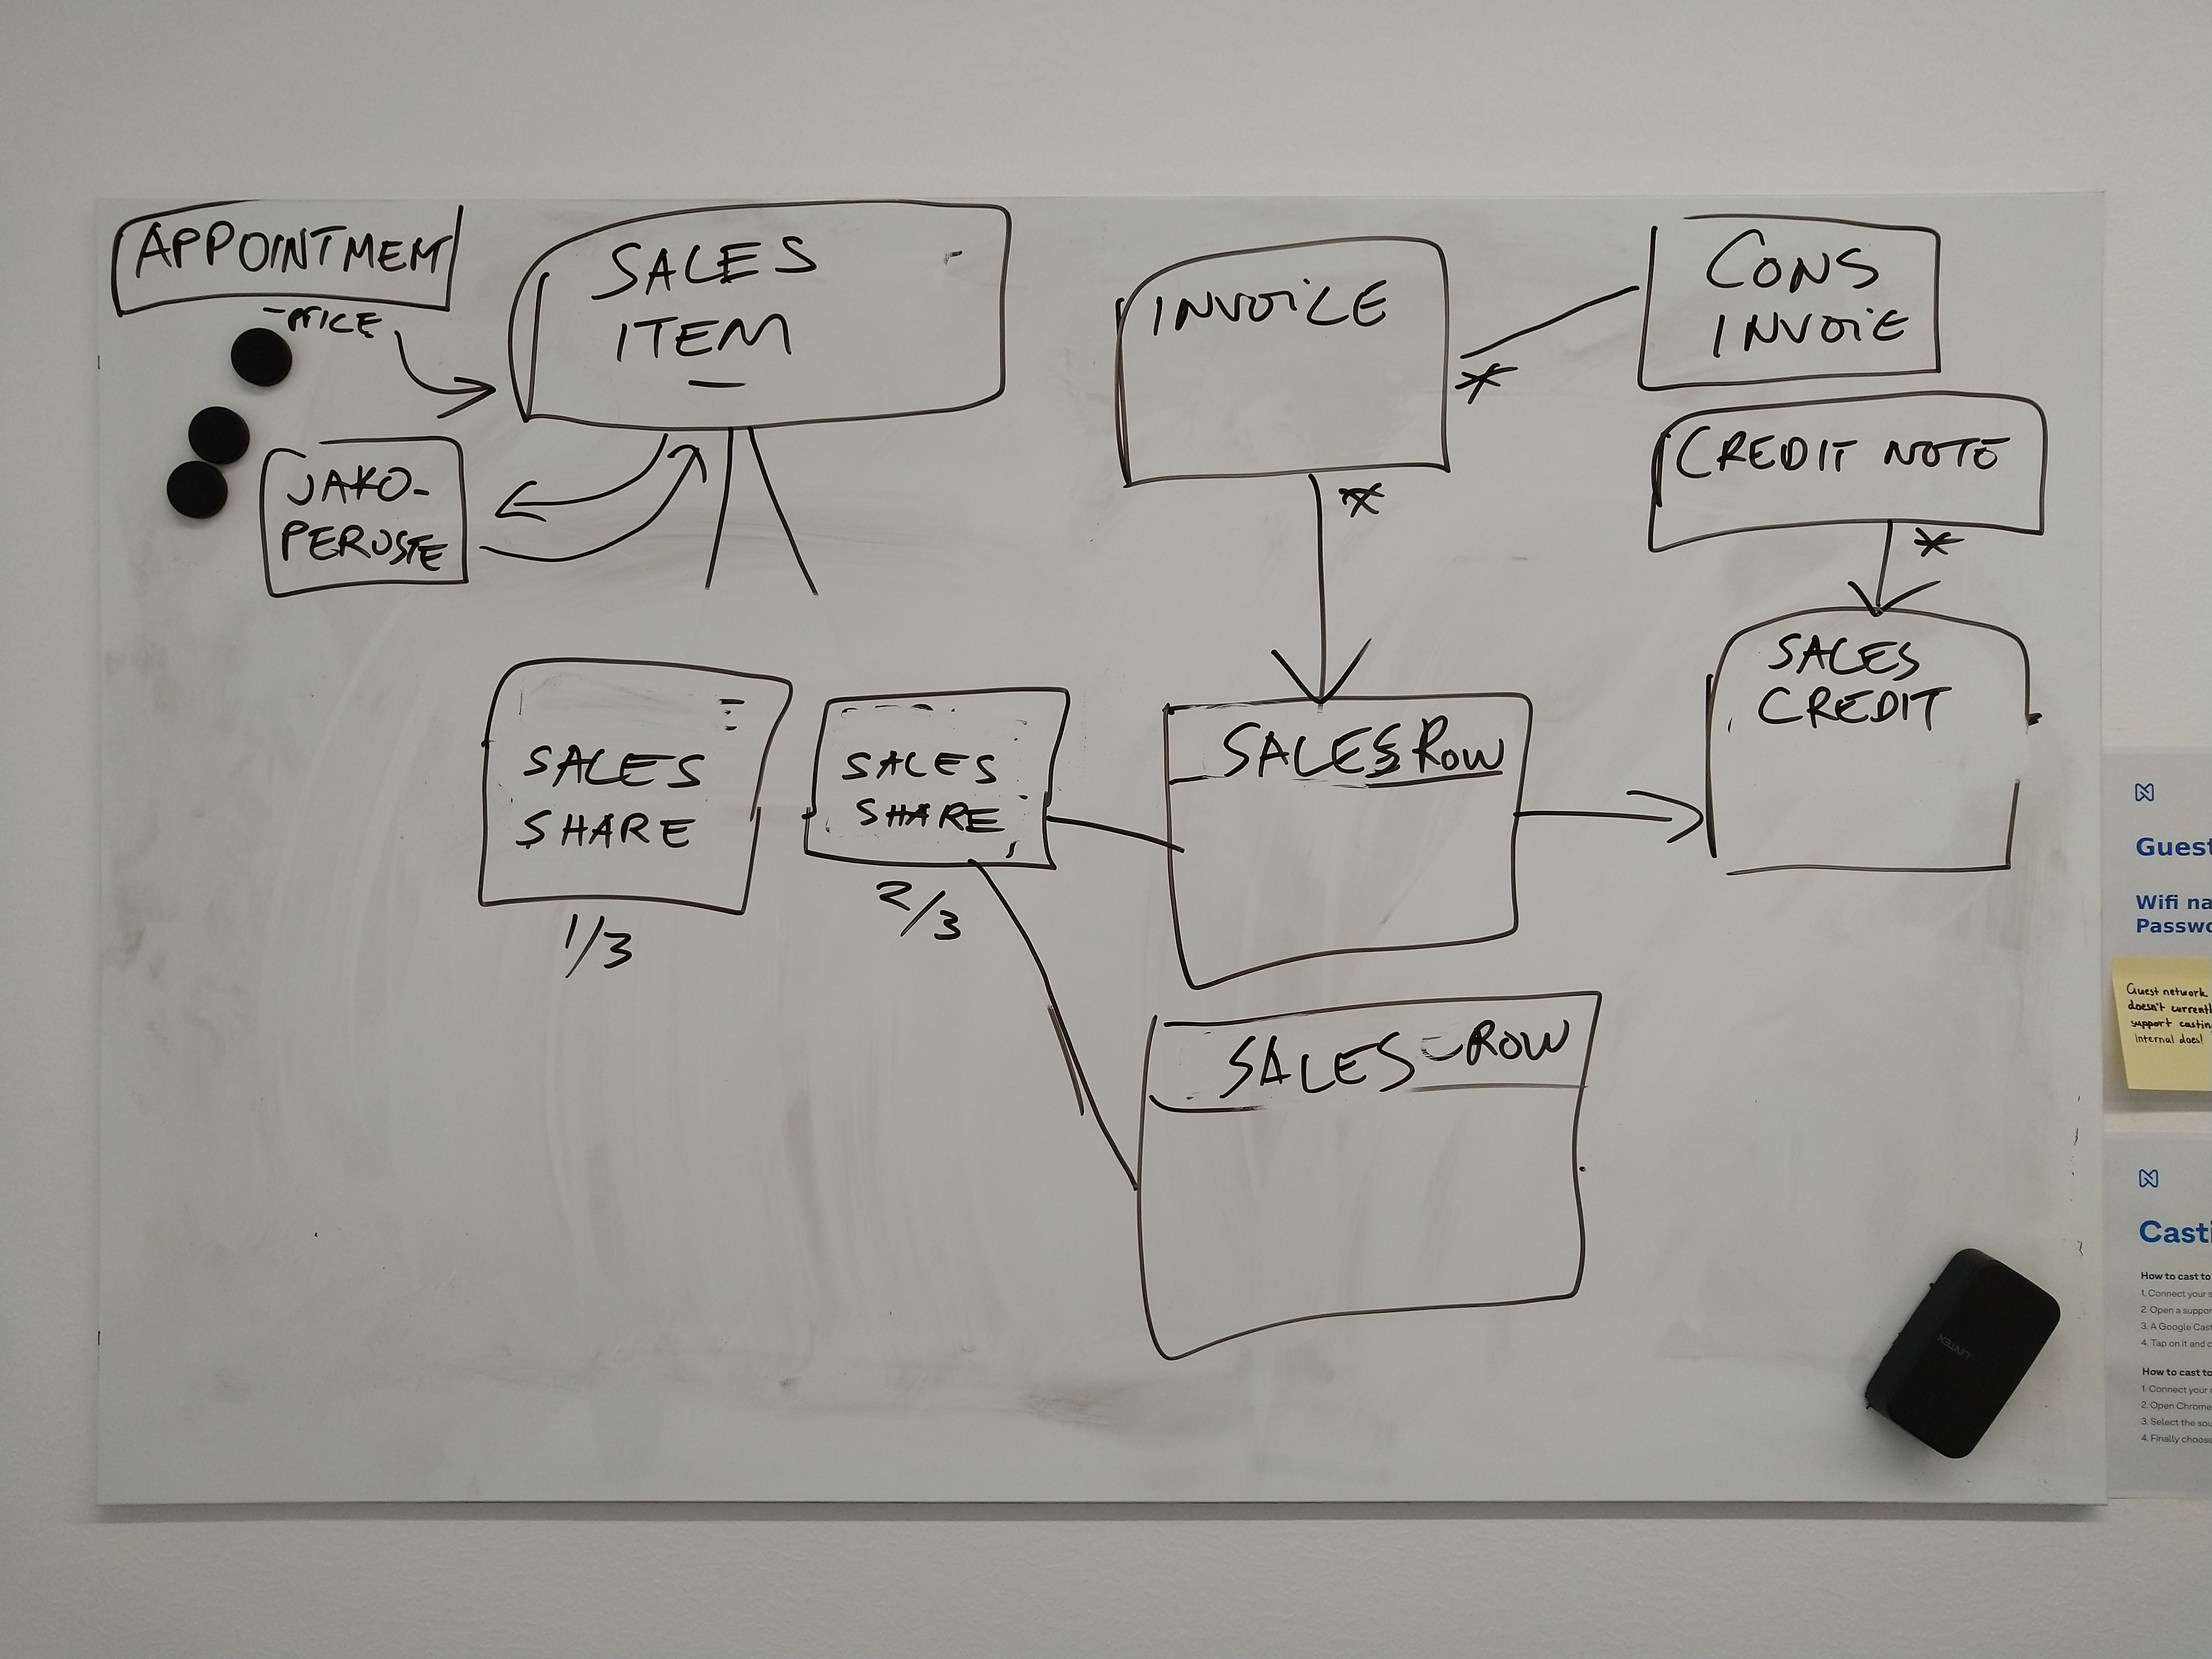
\includegraphics[width=\textwidth,height=0.5\textheight]{illustration/malli4.jpg}
\caption{\label{malli3}Kolmas malli}
\end{figure}

Kokouksen jälkeen ryhdyin muuttamaan ohjelmaa tämän uuden logiikan
mukaiseksi. Tämä vaati erittäin laajoja koodimuutoksia, ja vei kaikkiaan
kaksi päivää.

Uusien ominaisuuksien toteuttaminen refaktoroinnin jälkeen oli
suoraviivaista, ja tuloksena syntyi ohjelma, joka pääsi alkuperäiseen
tavoitteeseensa, jaetun käynnin hyvittämiseen ja uudelleen
laskuttamiseen.

\hypertarget{refaktorointi}{%
\section{Refaktorointi}\label{refaktorointi}}

Jouduin tekemään voimakkaita refaktorointeja jokaisen iteraation
taitteessa. Näistä en olisi selvinnyt ilman kattavia yksikkötestejä.

\hypertarget{kuxe4ytuxe4nnuxf6ssuxe4}{%
\section{\texorpdfstring{\Gls{ubilang}
käytännössä}{ käytännössä}}\label{kuxe4ytuxe4nnuxf6ssuxe4}}

Kuuluisivatkohan nämä oikeastaan tulosten tarkastelun tai yhteenvedon
alle?

Pitäessäni suunnittelukokouksia yhdessä tuoteomistajan kanssa, pyrin
koko ajan kuuntelemaan tarkalla korvalla, minkälaisia sanoja käytimme.
Tällä tavoin onnistuin nappaamaan joitain tärkeitä käsitteitä, joita
pystyi käyttämään mallin pohjana. Toisen kokouksemme aikana esiin
noussut \textbf{Laskutusperuste} oli juuri tällainen käsite.

Eric Evans mainitsee, että \textbf{Kaikenkattavan kielen} rakentamisessa
oleellista on löytää sanat, joita alan asiantuntijat käyttävät.

\hypertarget{kuxe4sitekarttojen-ja-graphql-skeeman-yhteys}{%
\section{Käsitekarttojen ja GraphQL-skeeman
yhteys}\label{kuxe4sitekarttojen-ja-graphql-skeeman-yhteys}}

Olin yllättynyt, miten täsmällisesti piirtämäni käsitekartat oli
mahdollista ilmaista GraphQL-skeeman avulla. Olioiden suhteet siirtyivät
vaivattomasti skeeman sisälle hierarkioiksi.
